\chapter{الجهد البدني وحاجات الجسم الطاقية}\label{ch:g10:exercise-and-energy}

دراجة تدوس على دراجة مختبرية في مقابل مكبح يقيس استطاعتها:
\qty{100}{W}، ثم \qty{150}{W}، ثم \qty{200}{W}. وقناع على وجهها يرسل
كل نفس إلى محلل. والأرقام على الشاشة تتسلق مع المكبح: فكلما زاد الشغل
الميكانيكي الذي تقدمه، زاد الأكسجين الذي تستهلكه وزاد ثاني أكسيد
الكربون الذي تزفره. عضلاتها تدير تنفس
\cref{ch:g10:cell-metabolism} بأقصى طاقته، والمحلل يقرأ ميزانيته.
ويتابع هذا الفصل طاقة الجهد البدني من الغذاء الذي يقدمها إلى الأكسجين
الذي يحررها.

\section{طاقة تدخل، وشغل يخرج}

\begin{definition}[الإنفاق الطاقي]\label{def:g10:exercise-and-energy:expenditure}
\emph{الإنفاق الطاقي}\index{إنفاق طاقي} للجسم، بالجول، هو مجموع الطاقة
التي تحررها خلاياه من الجزيئات العضوية في زمن معطى. ومقسومًا على
الزمن، يكون \emph{استطاعة استقلابية}، بالواط. ويصرف البالغ في الراحة
نحو \qty{80}{W} --- أي نحو \qty{7000}{kJ} في اليوم --- ليبقي القلب
نابضًا والدماغ عاملًا والحرارة عند \qty{37}{\celsius} \omterm{def:g10:cells-common-unit:cell}{والخلايا} حية؛
وهذا هو \emph{\omterm{def:g10:cell-metabolism:metabolism}{الاستقلاب} الأساسي}. وكل نشاط يضاف إليه.
\end{definition}

\begin{proposition}[أين تذهب الطاقة]\label{prop:g10:exercise-and-energy:efficiency}
العضلة العاملة لا تحول إلى شغل ميكانيكي إلا نحو ربع الطاقة التي
تحررها؛ أما الأرباع الثلاثة الأخرى فتغادر حرارةً. ومن ثم فتقديم
استطاعة ميكانيكية $P$ يكلف الجسم استطاعة استقلابية تقارب $4P$ فوق
الراحة: فالدراجة عند \qty{100}{W} على الدواستين تصرف نحو
\qty{400}{W} في عضلاتها، وعلى جسمها أن يتخلص من \qty{300}{W} حرارةً
--- بالتعرق في معظمه.
\end{proposition}
\admitted

\begin{example}[ميزانيات يومية]\label{ex:g10:exercise-and-energy:budgets}
تلميذ يجلس في الصف، ويمشي إلى المدرسة، وينام، يصرف نحو \qty{9000}{kJ}
في اليوم؛ وساعة من كرة القدم تضيف نحو \qty{2500}{kJ}؛ ويوم في الجبل
بحقيبة، \qty{15000}{kJ} إجمالًا. أما دراجة في مرحلة جبلية من سباق
فتصرف \qty{25000}{kJ}، ولا تستطيع أن تأكل في اليوم ما يغطيها. والطاقة
تأتي من الغذاء (\cref{ch:g10:chemistry-of-life}): \qty{17}{kJ} لكل
غرام من \omterm{def:g10:chemistry-of-life:families}{الكربوهيدرات} أو \omterm{def:g10:chemistry-of-life:families}{البروتين}، و\qty{38}{kJ} لكل غرام من الدهن.
\end{example}

\section{استهلاك الأكسجين يقيس الإنفاق الطاقي}

\begin{proposition}[المكافئ الأكسجيني]\label{prop:g10:exercise-and-energy:oxygen}
لما كانت طاقة الجهد البدني يحررها \omterm{prop:g10:cell-metabolism:respiration}{التنفس الخلوي}، وهو يستهلك الأكسجين،
كان استهلاك الجسم من الأكسجين يقيس إنفاقه الطاقي: فكل لتر من الأكسجين
المستهلك يقابل نحو \qty{20}{kJ} محررة، أيًّا كان خليط الغلوكوز
\omterm{def:g10:chemistry-of-life:families}{والدهون} المحروق. ويستهلك الإنسان في الراحة نحو \qty{0.25}{L} من
الأكسجين في الدقيقة؛ وأثناء الجهد يرتفع الاستهلاك تناسبًا مع
الاستطاعة المقدمة، حتى سقف شخصي.
\end{proposition}
\begin{proof}[شواهد]
تعطي معادلة التنفس في \cref{ch:g10:cell-metabolism} \qty{2870}{kJ}
لكل \qty{6}{mol} من الأكسجين، أي \qty{478}{kJ} للمول، ويشغل مول الغاز
نحو \qty{24}{L}: أي \qty{20}{kJ} للتر. والرقم عند \omterm{def:g10:chemistry-of-life:families}{الدهون}
\qty{19.6}{kJ/L}، وعند \omterm{def:g10:chemistry-of-life:families}{الكربوهيدرات} \qty{21.1}{kJ/L}، فالخليط لا
يكاد يهم. والقياسات في حجرات محكمة، تجمع فيها الحرارة التي يحررها
شخص جمعًا مباشرًا، توافق الرقم الأكسجيني في حدود بضعة بالمئة.
\end{proof}

\begin{omfigure}
\begin{tikzpicture}
\begin{axis}[
  width=0.86\linewidth, height=5.8cm,
  axis x line=bottom, axis y line=left,
  xmin=0, xmax=320, ymin=0, ymax=4.2,
  xlabel={الاستطاعة الميكانيكية (W)}, ylabel={$\mathrm{O_2}$ المستهلك (L/min)},
  xlabel style={font=\small, at={(axis description cs:0.5,-0.12)}, anchor=north},
  ylabel style={font=\small},
  tick label style={font=\small},
  xtick={0,50,100,150,200,250,300}, ytick={0,1,2,3,4},
  clip=false,
]
\addplot[thick, omThm, mark=*, mark size=1.6pt] coordinates
  {(0,0.3) (50,0.9) (100,1.5) (150,2.1) (200,2.7) (250,3.2) (300,3.3)};
\draw[dashed, gray] (axis cs:0,3.3) -- (axis cs:320,3.3);
\node[font=\small, anchor=south east] at (axis cs:318,3.32) {$\dot V\!\mathrm{O_2}$max};
\node[font=\small, anchor=south west, align=left] at (axis cs:40,3.42) {الميل: \qty{12}{mL} من $\mathrm{O_2}$ في الدقيقة\\ لكل واط};
\end{axis}
\end{tikzpicture}

{\small استهلاك الأكسجين عند شخص يدوس باستطاعة متزايدة. والارتفاع خطي
--- نحو \qty{12}{mL} من الأكسجين في الدقيقة لكل واط --- حتى يبلغ
الاستهلاك سقفه، وهو $\dot V\!\mathrm{O_2}$max عند ذلك الشخص؛ وما
وراءه تقدَّم الاستطاعة الزائدة من دون أكسجين ولا يمكن إدامتها.}
\end{omfigure}

\begin{definition}[الاستهلاك الأقصى للأكسجين]\label{def:g10:exercise-and-energy:vo2max}
\emph{الاستهلاك الأقصى للأكسجين}\index{استهلاك أقصى للأكسجين}، ويكتب
$\dot V\!\mathrm{O_2}$max، هو أعلى نسبة يستطيع بها جسم إنسان أن يأخذ
الأكسجين ويستعمله، باللترات في الدقيقة --- أو، لمقارنة أشخاص مختلفي
الأحجام، بالمليلترات في الدقيقة لكل كيلوغرام من كتلة الجسم. وهو يحدد
أعلى استطاعة يستطيع التنفس وحده إدامتها. ومن قيمه النموذجية:
\qty{35}{mL/min} لكل كيلوغرام عند بالغ قليل الحركة، و\num{50} عند
تلميذ مدرَّب، و\num{80} أو أكثر عند بطل في رياضات التحمل.
\end{definition}

\begin{example}[قراءة المنحني]\label{ex:g10:exercise-and-energy:reading}
في الشكل، تكلف \qty{100}{W} من الدوس \qty{1.5}{L/min} من الأكسجين:
أي $1.5 \times 20 = \qty{30}{kJ}$ في الدقيقة، وهو \qty{500}{W} من
الاستطاعة الاستقلابية --- أي \qty{100}{W} من الشغل زائد \qty{400}{W}
من الحرارة وحاجات الراحة، بما يوافق
\cref{prop:g10:exercise-and-energy:efficiency}. وسقف
\qty{3.3}{L/min} عند شخص كتلته \qty{66}{kg} هو \qty{50}{mL/min} لكل
كيلوغرام.
\end{example}

\begin{omfigure}
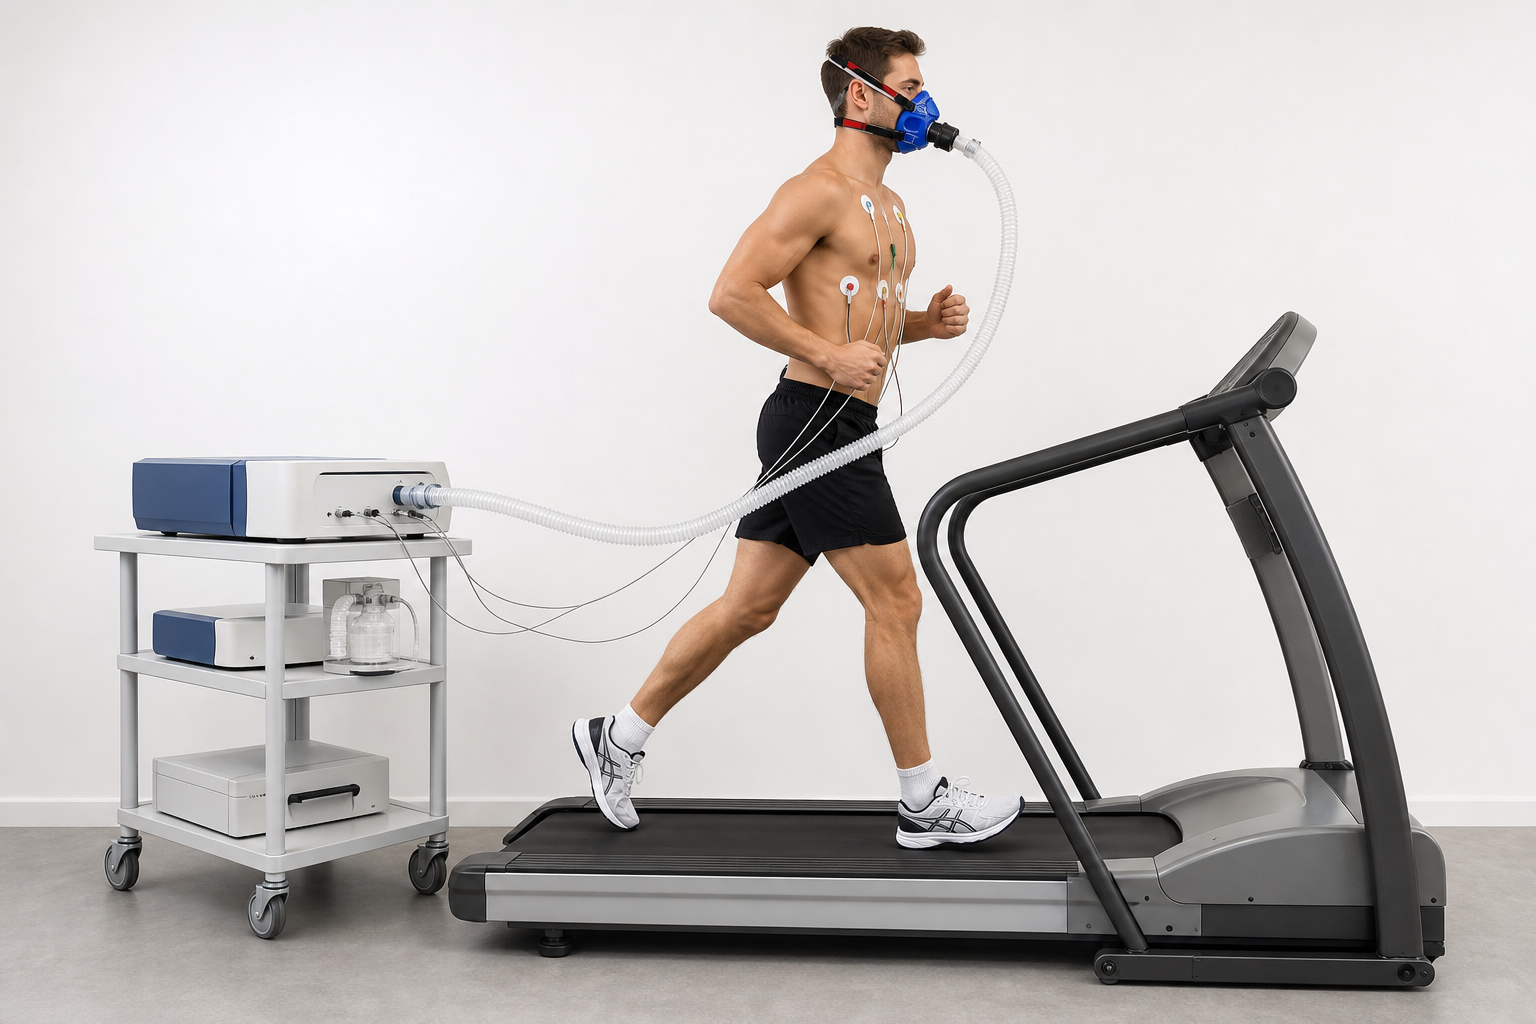
\includegraphics[width=0.62\linewidth]{images/book2/ai/g10-exercise-treadmill-mask.png}

{\small قياس استهلاك الأكسجين أثناء الجهد: كل نفس يمر عبر القناع إلى
محلل غازات يسجل الأكسجين المأخوذ وثاني أكسيد الكربون المطروح، دقيقة
بدقيقة، بينما يضبط بساط الجري الاستطاعة.}
\end{omfigure}

\section{وقود العضلة}

\begin{proposition}[ثلاثة مصادر لجزيء ATP]\label{prop:g10:exercise-and-energy:fuels}
تقلص العضلة يدفع ثمنه من ATP، \omterm{def:g10:cells-common-unit:cell}{والخلية} لا تحتفظ منه إلا بما يكفي بضع
ثوان. وهو يجدَّد بثلاثة طرق، لكل منها سرعته وسعته:
\begin{itemize}
  \item مخزون صغير من مركب فوسفاتي في العضلة، يعيد تكوين ATP في الحال
        لكنه يدوم نحو عشر ثوان --- وهو العدو السريع؛
  \item \omterm{def:g10:cell-metabolism:fermentation}{التخمر} اللبني للغلوكوز في \omterm{def:g10:cells-common-unit:cell}{السيتوبلازم}، وهو سريع لكنه مبدد،
        يديم جهدًا أقصى دقيقة إلى دقيقتين وينتج حمضًا لبنيًا؛
  \item \omterm{prop:g10:cell-metabolism:respiration}{التنفس الخلوي} في \omterm{def:g10:cells-common-unit:organelle}{المتقدرات}، وهو أبطأ في بلوغ نسبته القصوى
        لكنه غير محدود المدة تقريبًا، يحرق الغلوكوز من الدم،
        \omterm{def:g10:exercise-and-energy:glycogen}{والغليكوجين} من العضلة، والحموض الدهنية من شحم الجسم.
\end{itemize}
ويتوقف نصيب كل منها على شدة الجهد ومدته.
\end{proposition}
\admitted

\begin{omfigure}
\begin{tikzpicture}
\begin{axis}[
  ybar stacked, bar width=18pt,
  width=0.86\linewidth, height=5.6cm,
  axis x line=bottom, axis y line=left,
  ymin=0, ymax=100, ylabel={نصيب من الطاقة (\%)}, ylabel style={font=\small},
  symbolic x coords={10 s, 1 min, 4 min, 30 min, 2 h},
  xtick=data, tick label style={font=\small},
  xlabel={مدة جهد أقصى},
  xlabel style={font=\small, at={(axis description cs:0.5,-0.12)}, anchor=north},
  enlarge x limits=0.15,
  legend style={at={(0.5,-0.3)}, anchor=north, legend columns=3,
                font=\small, draw=none},
]
\addplot[fill=omThm!50, draw=omThm] coordinates {(10 s,85) (1 min,25) (4 min,8) (30 min,2) (2 h,1)};
\addplot[fill=omProp!50, draw=omProp] coordinates {(10 s,12) (1 min,50) (4 min,32) (30 min,8) (2 h,2)};
\addplot[fill=omDef!50, draw=omDef] coordinates {(10 s,3) (1 min,25) (4 min,60) (30 min,90) (2 h,97)};
\legend{{مخزون الفوسفات}, {التخمر اللبني}, {التنفس}}
\end{axis}
\end{tikzpicture}

{\small النصيب التقريبي لمصادر ATP الثلاثة في جهد أقصى مدته معطاة.
فعدو 100 متر يجري على مخزون الفوسفات؛ وسباق 400 متر على \omterm{def:g10:cell-metabolism:fermentation}{التخمر} في
معظمه؛ وكل ما يتجاوز بضع دقائق على التنفس.}
\end{omfigure}

\begin{definition}[الغليكوجين]\label{def:g10:exercise-and-energy:glycogen}
\emph{الغليكوجين}\index{غليكوجين} هو الصورة الحيوانية \omterm{def:g10:chemistry-of-life:families}{للكربوهيدرات}
المخزونة: سلسلة متفرعة من وحدات الغلوكوز، تحفظ حبيبات في \omterm{def:g10:cells-common-unit:cell}{خلايا} العضلة
(نحو \qty{400}{g} عند البالغ) وفي الكبد (نحو \qty{100}{g}). وغليكوجين
العضلة يقود العضلة التي تخزنه؛ أما غليكوجين الكبد فيفكك إلى غلوكوز
يطلق في الدم، فيبقي غلوكوز الدم قرب \qty{1}{g/L} للدماغ وسائر النسج.
أما الشحم، المخزون في \omterm{def:g10:cells-common-unit:cell}{الخلايا} الشحمية، فهو الاحتياطي الأكبر بكثير
(\cref{ch:g10:chemistry-of-life})، لكنه لا يحرق إلا ببطء ولا يحرق إلا
بالأكسجين.
\end{definition}

\begin{example}[جدار الماراثون]\label{ex:g10:exercise-and-energy:wall}
يستهلك الجري نحو \qty{4}{kJ} لكل كيلوغرام من كتلة الجسم لكل كيلومتر؛
فعدّاء كتلته \qty{70}{kg} يصرف \qty{280}{kJ/km}، والماراثون يكلف
\qty{11800}{kJ}. ومخازن \omterm{def:g10:exercise-and-energy:glycogen}{الغليكوجين} تحمل نحو \qty{8500}{kJ}. فإذا حرق
العدّاء غليكوجينه سريعًا أكثر مما ينبغي، نفدت المخازن قرب الكيلومتر
الثلاثين؛ وعلى العضلات عندئذ أن تعتمد على الشحم، وهو يقدم الطاقة بنصف
النسبة بالكاد، فتنهار الوتيرة --- وهو ما يسمى «ارتطامًا بالجدار».
والعدّاؤون المدرَّبون يحرقون نصيبًا أكبر من الشحم منذ البداية،
ويأكلون \omterm{def:g10:chemistry-of-life:families}{الكربوهيدرات} أثناء السباق.
\end{example}

\begin{omfigure}
\begin{tikzpicture}[>=Stealth, font=\small,
  b/.style={draw, rounded corners, align=center, minimum height=0.9cm, text width=2.5cm}]
  \node[b, fill=omDef!12] (food) at (0,2.2) {الغذاء:\\ كربوهيدرات ودهون};
  \node[b, fill=omDef!12] (gly) at (0,0.6) {غليكوجين (العضلة\\ والكبد)، غلوكوز الدم};
  \node[b, fill=omDef!12] (fat) at (0,-1.0) {حموض دهنية\\ من شحم الجسم};
  \node[b, fill=omThm!12, minimum height=2.6cm] (mit) at (4.3,-0.2) {المتقدرات:\\ التنفس};
  \node[b, fill=omProp!15] (o2) at (4.3,2.2) {أكسجين، من\\ الرئتين والدم};
  \node[b, fill=omMeth!15] (atp) at (9.2,-0.2) {ATP};
  \node[b, fill=white] (work) at (12.5,0.8) {شغل العضلة\\ (نحو 25\%)};
  \node[b, fill=white] (heat) at (12.5,-1.2) {حرارة\\ (نحو 75\%)};
  \draw[->] (food) -- (gly);
  \draw[->] (food.west) to[bend right=40] (fat.west);
  \draw[->] (gly) -- (mit);
  \draw[->] (fat) -- (mit);
  \draw[->] (o2) -- (mit);
  \draw[->] (mit) -- node[above, font=\scriptsize] {$\mathrm{CO_2}$ يخرج} (atp);
  \draw[->] (atp) -- (work);
  \draw[->] (atp) -- (heat);
\end{tikzpicture}

{\small سلسلة الطاقة في جهد مستدام: وقود من الغذاء ومن مخازن الجسم،
وأكسجين من التنفس، وATP يصنع في \omterm{def:g10:cells-common-unit:organelle}{المتقدرات} ويصرف على التقلص --- ثلاثة
أرباعه تغادر حرارةً.}
\end{omfigure}

\section{القياس والاستدلال}

\begin{method}[حساب طاقي لجهد بدني]\label{met:g10:exercise-and-energy:calc}
\begin{enumerate}
  \item من الأكسجين: الطاقة (\unit{kJ}) $=$ الأكسجين المستهلك
        (\unit{L}) $\times 20$. واطرح استهلاك الراحة إذا كان السؤال
        عن كلفة الجهد وحده.
  \item من الاستطاعة الميكانيكية: الاستطاعة الاستقلابية
        $\approx 4 P$؛ والطاقة $=$ الاستطاعة $\times$ الزمن
        (\qty{1}{W} في \qty{1}{s} هي \qty{1}{J}؛ و\qty{1}{kWh}
        $= \qty{3600}{kJ}$).
  \item من الوقود: الكتلة المحروقة $=$ الطاقة $/$ القيمة الطاقية
        (\qty{17}{kJ/g} \omterm{def:g10:chemistry-of-life:families}{للكربوهيدرات}، و\qty{38}{kJ/g} للدهن)؛
        \omterm{def:g10:exercise-and-energy:glycogen}{والغليكوجين} مخزون مع ثلاثة أمثال كتلته ماءً.
  \item تحقق من رتب القدر: فاليوم كله نحو \qty{10000}{kJ}؛ والساعة
        الشاقة \qtyrange{2000}{3000}{kJ}؛ والماراثون
        \qty{12000}{kJ}.
\end{enumerate}
\end{method}

\begin{example}[ساعة من ركوب الدراجة]\label{ex:g10:exercise-and-energy:hour}
ساعة واحدة عند \qty{150}{W} على الدواستين: الاستطاعة الاستقلابية نحو
\qty{600}{W}، والطاقة $600 \times 3600 = \qty{2.16e6}{J} \approx
\qty{2200}{kJ}$؛ والأكسجين $2200/20 = \qty{110}{L}$، أي
\qty{1.8}{L/min} --- بما يوافق المنحني. فإذا جاء النصف من
\omterm{def:g10:chemistry-of-life:families}{الكربوهيدرات}: $1100/17 \approx \qty{65}{g}$ من الغلوكوز أو
\omterm{def:g10:exercise-and-energy:glycogen}{الغليكوجين}، و$1100/38 \approx \qty{29}{g}$ من الشحم.
\end{example}

\begin{remark}[لماذا يجب أن يصل الأكسجين]\label{rem:g10:exercise-and-energy:delivery}
كل ما تقدم يفترض أن الأكسجين يبلغ \omterm{def:g10:cells-common-unit:organelle}{المتقدرات} بالسرعة التي تستطيع بها
استعماله. وتلك مهمة الرئتين والقلب والدم، واستجابتها للجهد --- تنفس
أسرع، ونبض أسرع وأقوى، ودم يوجه إلى العضلات --- موضوع
\cref{ch:g10:heart-lungs-effort}. و$\dot V\!\mathrm{O_2}$max حد في
الإيصال في معظمه، لا في شهية العضلات.
\end{remark}

\section{تمارين}

\begin{exercise}[$\star$]\label{exo:g10:exercise-and-energy:1}
عرّف \omterm{def:g10:cell-metabolism:metabolism}{الاستقلاب} الأساسي وأعطِ رتبة قدره بالواط وبالكيلوجول في اليوم.
\end{exercise}

\begin{exercise}[$\star$]\label{exo:g10:exercise-and-energy:2}
شخص يستهلك \qty{2.0}{L} من الأكسجين في الدقيقة. ما إنفاقه الطاقي
بالكيلوجول في الدقيقة، وبالواط؟
\end{exercise}

\begin{exercise}[$\star$]\label{exo:g10:exercise-and-energy:3}
سمِّ الطرق الثلاثة التي تجدد بها العضلة ATP فيها وأعطِ المدة
النموذجية التي يستطيع كل منها إدامتها وحده.
\end{exercise}

\begin{exercise}[$\star$]\label{exo:g10:exercise-and-energy:4}
ما $\dot V\!\mathrm{O_2}$max؟ حوّل \qty{3.5}{L/min} عند شخص كتلته
\qty{70}{kg} إلى مليلترات في الدقيقة لكل كيلوغرام.
\end{exercise}

\begin{exercise}[$\star$]\label{exo:g10:exercise-and-energy:5}
أين يخزن \omterm{def:g10:exercise-and-energy:glycogen}{الغليكوجين}، وبأي مقادير، وفيم يستعمل كل مخزن؟
\end{exercise}

\begin{exercise}[$\star\star$]\label{exo:g10:exercise-and-energy:6}
من شكل الأكسجين بدلالة الاستطاعة، اقرأ استهلاك الأكسجين عند
\qty{200}{W} واحسب الاستطاعة الاستقلابية. واستنتج الحرارة المنتجة في
الثانية.
\end{exercise}

\begin{exercise}[$\star\star$]\label{exo:g10:exercise-and-energy:7}
ماشٍ كتلته \qty{60}{kg} يصعد \qty{800}{m} في ساعتين. احسب الشغل
الميكانيكي ضد الثقالة ($g = \qty{9.8}{N/kg}$)، والطاقة التي صرفتها
عضلاته إذا كان المردود 25\%، والاستطاعة الاستقلابية الوسطية فوق
الراحة.
\end{exercise}

\begin{exercise}[$\star\star$]\label{exo:g10:exercise-and-energy:8}
باستعمال شكل الأعمدة المكدسة، فسّر لماذا يكون عدّاء 400 متر مبهورًا
موجعًا عند خط النهاية بينما يكاد عدّاء 100 متر لا يلهث.
\end{exercise}

\begin{exercise}[$\star\star$]\label{exo:g10:exercise-and-energy:9}
رياضية تصرف \qty{3000}{kJ} في حصة تدريب، 60\% منها من \omterm{def:g10:chemistry-of-life:families}{الكربوهيدرات}.
ما كتلة \omterm{def:g10:exercise-and-energy:glycogen}{الغليكوجين} التي استعملتها، وما كتلة الماء التي تحررت معه؟
\end{exercise}

\begin{exercise}[$\star\star$]\label{exo:g10:exercise-and-energy:10}
لوح شوكولاتة كتلته \qty{50}{g} يقدم \qty{1100}{kJ}. فكم من الوقت يقود
دراجًا يدوس عند \qty{150}{W}؟
\end{exercise}

\begin{exercise}[$\star\star$]\label{exo:g10:exercise-and-energy:11}
لماذا ترتفع حرارة جسم الإنسان أثناء الجهد، وبأي آلية يمنع من الارتفاع
أكثر؟
\end{exercise}

\begin{exercise}[$\star\star\star$]\label{exo:g10:exercise-and-energy:12}
شخصان كتلتاهما \qty{60}{kg} و\qty{90}{kg} ولكليهما
$\dot V\!\mathrm{O_2}$max يبلغ \qty{3.6}{L/min}. أيهما يستطيع الجري
صعودًا أسرع، وأيهما يستطيع الدوس أقوى على طريق مستوٍ على دراجة
مختبرية؟ فسّر.
\end{exercise}

\begin{exercise}[$\star\star\star$]\label{exo:g10:exercise-and-energy:13}
استهلاك عدّاء من الأكسجين أثناء سباق هو \qty{3.0}{L/min} بوتيرة تقتضي،
بحسب المنحني، \qty{3.4}{L/min}. فمن أين يأتي الفرق، وماذا سيشعر
العدّاء بعد بضع دقائق؟
\end{exercise}

\begin{exercise}[$\star\star\star$]\label{exo:g10:exercise-and-energy:14}
فسّر، بالطرق الثلاثة لتجديد ATP، لماذا لا يستطيع الإنسان أن يفقد
الشحم بجهد أقصى في نوبات قصيرة بفعالية ما يفقده بجهد معتدل طويل
المدة.
\end{exercise}

\begin{exercise}[$\star\star\star$]\label{exo:g10:exercise-and-energy:15}
دراجة في مرحلة جبلية تصرف \qty{25000}{kJ} في يوم. وغليكوجينها يحمل
\qty{8500}{kJ} وتأكل \qty{6000}{kJ} أثناء المرحلة. قدّر كتلة شحم
الجسم التي تحرقها، وفسّر لماذا يأكل الدراجون باستمرار في مثل هذه
المرحلة.
\end{exercise}

\section{مسألة: أين يقف الجدار}

\begin{problem}[{مسألة نهاية الأسبوع --- ميزانية ماراثون الطاقية:
الأكسجين الذي تتنفسه العدّاءة، والغليكوجين الذي تحمله، والكيلومتر الذي
ينفد عنده، وما الذي يغيره التدريب}]
\label{pb:g10:exercise-and-energy:1}
نادية، \qty{60}{kg}، تجري ماراثونًا (\qty{42.2}{km}) في
\qty{3}{h}\,\qty{30}{min}. والجري يكلف \qty{4.0}{kJ} لكل كيلوغرام لكل
كيلومتر. وعضلاتها تحمل \qty{300}{g} من \omterm{def:g10:exercise-and-energy:glycogen}{الغليكوجين} وكبدها \qty{80}{g}؛
\omterm{def:g10:exercise-and-energy:glycogen}{والغليكوجين} والغلوكوز يعطيان \qty{17}{kJ/g}، والشحم \qty{38}{kJ/g}؛
ولتر الأكسجين الواحد يحرر \qty{20}{kJ}. و$\dot V\!\mathrm{O_2}$max
عندها \qty{52}{mL/min} لكل كيلوغرام.

\medskip
\noindent\textbf{الجزء الأول --- كلفة السباق.}
\begin{enumerate}
  \item احسب الكلفة الطاقية للماراثون عند نادية.
  \item احسب استطاعتها الاستقلابية الوسطية أثناء السباق، بالواط.
  \item احسب حجم الأكسجين الذي تستهلكه عبر السباق، ثم استهلاكها
        الوسطي للأكسجين باللترات في الدقيقة.
  \item عبّر عن ذلك الاستهلاك بالمليلترات في الدقيقة لكل كيلوغرام،
        وبنسبة مئوية من $\dot V\!\mathrm{O_2}$max عندها.
  \item استهلاكها في الراحة \qty{0.2}{L/min}. فأي نسبة من استهلاك يوم
        السباق يفسرها الجري نفسه؟
\end{enumerate}

\medskip
\noindent\textbf{الجزء الثاني --- المخازن.}
\begin{enumerate}[resume]
  \item احسب الطاقة المحفوظة في مخازن غليكوجينها.
  \item لو أنها حرقت \omterm{def:g10:exercise-and-energy:glycogen}{الغليكوجين} وحده، فعند أي كيلومتر تنفد المخازن؟
  \item والحق أنها تحرق خليطًا: 80\% \omterm{def:g10:chemistry-of-life:families}{كربوهيدرات} و20\% شحمًا بوتيرة
        سباقها. فعند أي كيلومتر ينفد \omterm{def:g10:exercise-and-energy:glycogen}{الغليكوجين} الآن؟
  \item ما كتلة الشحم التي تحرقها في السباق؟ قارنها بكتلة \qty{9}{kg} من
        الشحم تحملها عادةً امرأة كتلتها \qty{60}{kg}.
  \item فسّر، انطلاقًا من \cref{prop:g10:exercise-and-energy:fuels}،
        لماذا لا تستطيع ببساطة أن تحرق الشحم وحده حالما ينفد
        \omterm{def:g10:exercise-and-energy:glycogen}{الغليكوجين} وتحافظ على الوتيرة نفسها.
\end{enumerate}

\medskip
\noindent\textbf{الجزء الثالث --- التغلب على الجدار.}
\begin{enumerate}[resume]
  \item تشرب أثناء السباق محلولًا سكريًا يقدم \qty{60}{g} من
        \omterm{def:g10:chemistry-of-life:families}{الكربوهيدرات} في الساعة. فكم طاقة يضيف ذلك عبر السباق، وكم
        كيلومترًا من استعمال \omterm{def:g10:chemistry-of-life:families}{الكربوهيدرات} يغطي؟
  \item أعد السؤال 8 مع المشروب. فهل تنهي السباق الآن قبل نفاد
        \omterm{def:g10:exercise-and-energy:glycogen}{الغليكوجين}؟
  \item قبل السباق بثلاثة أيام «تشحن» \omterm{def:g10:chemistry-of-life:families}{الكربوهيدرات}، فترفع \omterm{def:g10:exercise-and-energy:glycogen}{غليكوجين}
        عضلاتها إلى \qty{500}{g}. وكل غرام مخزون مع \qty{3}{g} من
        الماء. فبكم ترتفع كتلتها، وما كلفة ذلك طاقةً لكل كيلومتر؟
  \item يزيح التدريب خليط وتيرة سباقها إلى 55\% \omterm{def:g10:chemistry-of-life:families}{كربوهيدرات} و45\%
        شحمًا. فمع الشحن والمشروب، عند أي كيلومتر ينفد \omterm{def:g10:exercise-and-energy:glycogen}{الغليكوجين}؟
        علّق.
  \item لماذا يجعل الدماغ، وهو لا يستعمل إلا الغلوكوز، نفادَ
        \omterm{def:g10:exercise-and-energy:glycogen}{الغليكوجين} يحس إنهاكًا حتى حين يبقى عند العضلات شحم تحرقه؟
\end{enumerate}

\medskip
\noindent\textbf{الجزء الرابع --- أرقام بطل.}
عدّاء نخبة كتلته \qty{55}{kg} يجري الماراثون في \qty{2}{h}\,
\qty{05}{min}، وكلفة جريه \qty{3.6}{kJ} لكل كيلوغرام لكل كيلومتر
و$\dot V\!\mathrm{O_2}$max عنده \qty{80}{mL/min} لكل كيلوغرام.
\begin{enumerate}[resume]
  \item احسب الكلفة الطاقية للسباق عند البطل واستهلاكه الوسطي
        للأكسجين باللترات في الدقيقة.
  \item أي نسبة مئوية من $\dot V\!\mathrm{O_2}$max عنده يديمها؟
        قارنها برقم نادية.
  \item يميز البطلَ أمران: سقف أعلى وكلفة أدنى لكل كيلومتر. فأيهما
        هو «الاقتصاد»؟ واحسب بكم يغير فرق الكلفة وحده طاقة السباق
        عند عدّاء كتلته \qty{55}{kg}.
  \item تحمل عضلاته \qty{500}{g} من \omterm{def:g10:exercise-and-energy:glycogen}{الغليكوجين} بعد الشحن. فعند
        استعمال 70\% \omterm{def:g10:chemistry-of-life:families}{كربوهيدرات}، هل يبلغ خط النهاية عليه من دون شرب؟
  \item اذكر النتيجة: عند نادية، الكيلومتر الذي يقف عنده الجدار بلا
        استعداد، والتدابير الثلاثة التي تزحزحه وراء خط النهاية.
\end{enumerate}
\end{problem}
